%Physics: EnergyCons, PE, KE
%Maths: Trig
\begin{problem}[Phil_Masses_Slope] 
{A particle $A$ has mass $m$ and moves on a smooth plane inclined at an angle $\theta = 30^{\circ}$ to the horizontal. Particle $B$, with mass $2m$, is attached to it by a light inextensible string running over a smooth pulley at the top of the slope. The system is held in position with $B$ hanging vertically and the string taut. When the system is released, $B$ falls a vertical distance $x$, causing $A$ to move up the slope as in Figure \ref{fig:Dynamics_masses_slope_30}.
\begin{figure}[h]
	\centering
	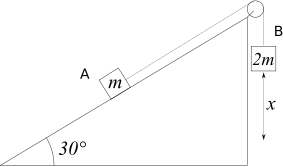
\includegraphics[width=0.3\textwidth]{Dynamics_masses_slope_30}
	\caption{}
	\label{fig:Dynamics_masses_slope_30}
\end{figure}
\nl
What is the speed of the particles after this motion?
\begin{enumerate}
	\item $\sqrt{\frac{5}{3}gx}$
	\item $\sqrt{\left(\frac{4 + \sqrt{3}}{3}\right)gx}$
	\item $\sqrt{\left(\frac{4 - \sqrt{3}}{3}\right)gx}$
	\item $\sqrt{gx}$
	\item $\sqrt{\frac{1}{2}gx}$
\end{enumerate}
}
{\textit{Created for the Rutherford School Physics Project by PS.}}
{The correct answer is (d). In this question, the gravitational potential energy lost by $B = 2mgx$. The gravitational potential energy gained by $A = mgx\sin{30^{\circ}} = \frac{1}{2}mgx$, so the total GPE lost $= 2mgx - \frac{1}{2}mgx = \frac{3}{2}mgx$. This is equal to the total kinetic energy gained by both particles: $\frac{1}{2}\left(3m\right)v^{2} = \frac{3}{2}mgx$. Rearrange this equation to obtain the answer.
}
\end{problem}